%\documentclass{sig-alternate}
\documentclass[11pt,twocolumn]{article}
\usepackage{url}
\usepackage{graphicx}
\usepackage{subfig}

%\newcommand{\IGNORE}[1]{}

\title{Summer Research Report}

%\numberofauthors{7}
\author{
  Bilawal Shaikh\\
  bilawal.shaikh@richmond.edu
}
\date{July 22, 2016}

\begin{document}

\maketitle
\begin{abstract}
  Neural Networks have been developed to provide machines with intelligence to choose and select, albeit not at par with humans. This requires choosing the right initial weights and biases, choosing the appropriate hyperparameters, etc. My job was to understand how this intelligence (machine learning) works so as to improve accuracy for machine recognition of bird images which were previously taken. I worked mostly on using image-augmentation techniques to increase the dataset which I found Lasagne is not really suitable for. Other attempts were made at improving accuracy such as using real-time augmentation using Keras, running the data set on Spark, and making various changes to the architecture.
  
\end{abstract}


\section{Introduction}

I was trying to increase the validation accuracy of the images by trying to change the architecture of the neural network and do basic image augmentation on the images. I used a dataset of 531 images, which later increased to 2655 images because of image augmentation techniques as shown below.

\begin{figure}
  \centering
  \subfloat[Original Image]{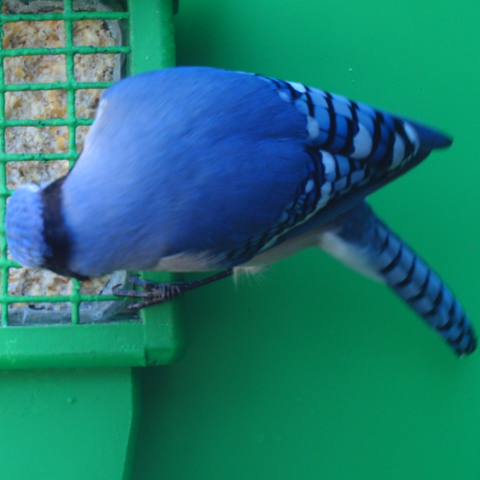
\includegraphics[width=0.5in]{2014-03-21_12_10.jpg}}
  \hspace*{1em}
  \subfloat[Image rotated by 17 degrees]{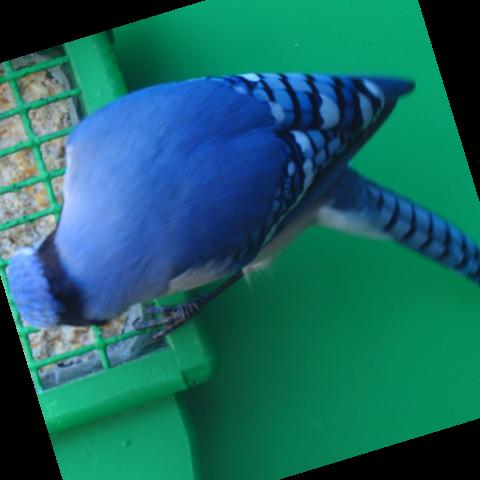
\includegraphics[width=0.5in]{rotation17.jpg}}
  \hspace*{1em}
  \subfloat[Image rotated by 34 degrees]{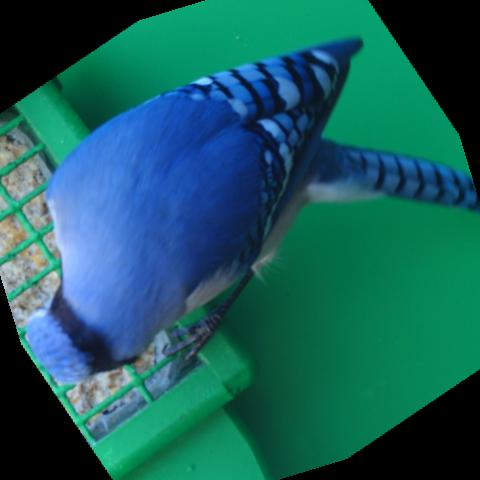
\includegraphics[width=0.5in]{rotation34.jpg}}
  \hspace*{1em}
  \subfloat[Image rotated by 50 degrees]{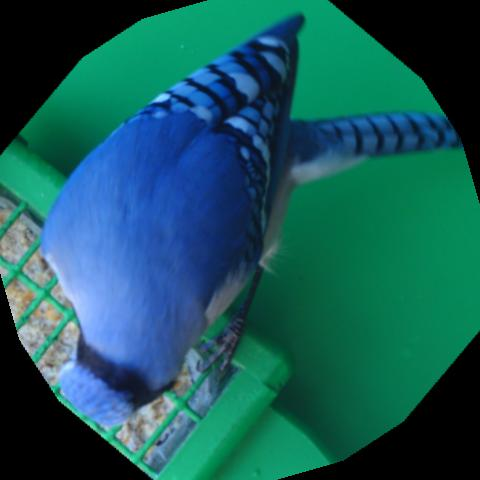
\includegraphics[width=0.5in]{rotation50.jpg}}
  \hspace*{1em}
  \subfloat[Image rotated by 62 degrees]{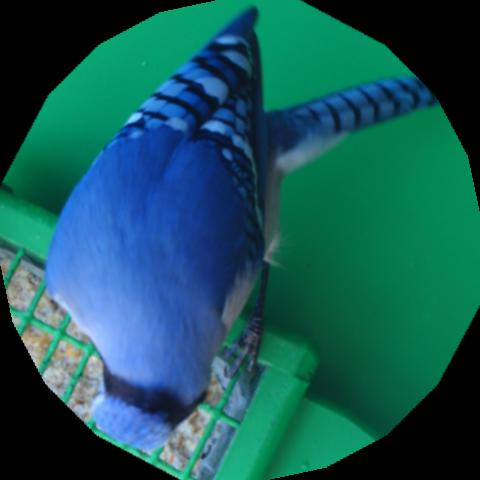
\includegraphics[width=0.5in]{rotation62.jpg}}
  \caption{example of how one image is augmented. \label{fig:TypicalImages}}
\end{figure}

Some of the contributions of this paper include: ran  the data on two separate configuration files, varied the learning rate between epochs, varied the number of repetitive layers in Dinc's configuration file, varied the value of hyperparameters in Dinc's configuation file, attempted to use Kera's real time image augmentation techniques on the data set, as well as adding noise layers on Dinc's code. 

In the end, I was limited by Lasagne's limitations of augmentation techniques and attempting to append the training images in the training set. The dataset with 2655 images took more than a day to run and more than 15 minutes just to show if the program has been debugged correctly or not, so working on a faster GPU would have saved a lot of time.

At the end of my research, I started learning about Spark and RDD's and how they are faster on very large datasets. But I abandoned this approach upon arriving on the conclusion that having large datatsets due to image augmentation was not helping in increasing accuracy. This approach may be helpful later when I use other machine learning libraries and use Keras' real-time augmentation techniques correctly.

\section{Related Work}


In \cite{BIRDID:Berg2013}, Berg and Belhumeur construct an image recognition
system with the goal of explaining to birders the differences between
similar species.

In \cite{BIRDID:Chatfield2014}, it was shown that data augmentation has benefits
to shallow feature encoding methods as well as neural networks. 

In \cite{BIRDID:duchi2011adaptive}, Duchi et al introduce the adagrad algorithm to 
modify the learning rate. This modifies the step size during gradient descent to achieve
better and faster training data results simply by setting an initial learning rate.

In \cite{BIRDID:fredembach2006}, shadow removal method were developed.

In \cite{BIRDID:Lecun2015}, the current state-of-the-art in deep learning techniques were 
reviewed by some of the leading figures in the field.
 

\section{Methods}
\label{sec:methods}

\paragraph{Image collection}

Images were collected using a Wingscapes BirdCam 2.0, a motion-activated
camera with maximum resolution of 8 megapixels. The images were collected
in Richmond, Virginia, USA, over a period of six months from
March through August of 2014. The images
were collected at the camera's medium resolution setting, producing images
that were 2048 x 1536 pixels. The target was an upright suet feeder with a
tail-prop, a configuration favored by woodpeckers. An opaque shield
was mounted behind the feeder to provide a uniform background for the
images. The shield and feeder were painted with Krylon Neon Green paint.
Neon green was chosen because none of the species that typically feed
as this type of feeder have any green in their plumage, making it more
difficult to confuse background pixels with pixels belonging to the
bird in background removal algorithms. The feeder, shield and camera
were mounted on a pole equipped with a squirrel baffle. The camera was
attached to the pole by an adjustable arm, sold as an accessory by
Wingscapes.

The camera has various settings controlling focus,  sensitivity to motion
and how the camera responds when motion is detected. The camera does not
autofocus; rather, it has a series of selectable fixed focus distances.
The shortest focus distance puts the focus point at approximately the
back of the feeder with the arm fully extended in our setup, which means
that, especially in low light situations where depth-of-field is shallow,
the bird is not in sharp focus. Experimentation revealed that the most
sensitive setting for motion detection was set off even by vibrations
in the shield caused by wind, resulting in hundreds of images of an
empty feeder. Consequently, the camera was set at medium sensitivity,
and was programmed to capture three images for each motion detected
event, followed by a 30 second pause before sensing for motion again.
Some species, like Carolina Chickadees and Tufted Titmice, perch,
procure a beak-full of food, and are off immediately. Other species,
such as Carolina Wrens and the woodpeckers, perch and stay on the
feeder for extended periods of time. As a result, the size of useful
training and validation sets were limited by the number of images
captured of the more shy species.

Not all species present in the area where the images were collected
visit feeders, and of those that do, not all visit the style of
feeder used in this study. A total of sixteen species visited
the feeding station during the data collection period. Of those,
nine species were present in enough images to be useful for
training and validating a classifer. The species used in the training
set is shown in Table \ref{table:species}.
\begin{table}[h]
  \caption{Training set species}
  \label{table:species}
  \begin{center}
    \begin{tabular}{l}
      \hline
      %\bf{Training set species} \\ \hline
      Blue Jay \\ 
      Brown Thrasher \\ 
      Carolina Chickadee \\ 
      Carolina Wren \\ 
      Downy Woodpecker  \\ 
      Northern Cardinal \\ 
      Red-bellied Woodpecker \\ 
      Tufted Titmouse \\ 
      Yellow Rumped Warbler \\ \hline
    \end{tabular}
  \end{center}
\end{table}
In some cases, a tenth category of images of an empty feeder
was added. In all reported results, each class consisted of 98 images.
Two typical images are show in figure \ref{fig:TypicalImages}.

\paragraph{Convolutional neural network architecture}

The Convolutional neural network architectures used the Lasagne machine learning library on top of the Theano machine learning library. I used two networks to do my calculations: one was the architecture provided by Dinc. Dinc's code used 1 padding layer, convolutional 2D layer, Max Pooling layer, and then another  padding layer, convolutional 2D layer, Max Pooling layer, this configuration was used to create a series of layers. The learning algorithm used for Dinc's code was adagrad with learning rate 0.009

The second one was alexnet which used Thang's code to run. Alexnet used one Convolution layer, one pooling layer, another convolution layer, then another pooling layer and then 2 convolution layers, then another pooling layer and lastly two Dense layers. The learning algorithm used for Alexnet's code was adadelta with learning rate 0.1 (this learning rate changes to the correct value as the program runs).

Both Dinc and Thang's code used numpy arrays for the data, and scipy for image augmentation (although I used skimage for image augmentation too but the results were similar). The code did differ on how the train$\_$fn and valid$\_$fn were being computed. 

\section{Results}
\label{sec:results}

Results are provided in the table below\footnote{The validation accuracy is given as a range by taking the minumum and maximum accuracy between epoch 250 and 300.}:

\begin{tabular}{ |p{5cm}||p{2.5cm}|  }
 \hline
 \multicolumn{2}{|c|}{Alexnet} \\
 \hline
 Changes to the code & validation accuracy/$\%$\\
 \hline
 Original code and configuration file&89.5-93.3\\
 \hline
 Using augmentation techniques to increase the dataset two-fold&90.0-93.8 \\
 \hline
 Using augmentation techniques to increase the dataset five-fold&89.4-93.5 \\
 \hline
 Changing the preaugmented dimensions of the image from 140x140 to 160x160&91.7-94.8 \\
 \hline
 Changing the preaugmented dimensions of the image from 140x140 to 200x200&91.1-95.1 \\
 \hline
\end{tabular}

\begin{tabular}{ |p{5cm}||p{2.8cm}|  }
 \hline
 \multicolumn{2}{|c|}{Dinc} \\
 \hline
 Changes to the code and configuration file & validation accuracy/$\%$\\
 \hline
 Original code and configuration file & 88.6-92.3 \\
 \hline
 Adding one more layer to the configuration file&86.9-91.7 \\
 \hline
 Adding two more layers to the original configuration&87.3-91.7  \\
 \hline
 Using augmentation techniques to increase the dataset two-fold&84.2-92.6 \\
 \hline
 Using augmentation techniques to increase the dataset five-fold&87.3-92.1 \\
 \hline
 Changing the preaugmented dimensions of the image from 140x140 to 160x160&85.2-92.2 \\
 \hline
 Changing the preaugmented dimensions of the image from 140x140 to 200x200&89.3-92.4 \\
 \hline
 Adding a Gaussian noise-layer after the input layer&0.758-0.796 \\
 \hline
 Changed all num$\_$filters in the layers by half&0.889-0.929 \\
 \hline
 Decreased the learning rate by a factor of 5 after epoch 150 and again by a factor of 5 after epoch 225 &0.882-0.914 \\
 \hline
\end{tabular}

\section{Discussion}

The results came because of the specific hyperparameters used, and the way the lasagne library computed the input layer. The rotation used in images did not increase accuracy maybe because of Lasagne overfits rotations, this point is reinforced due to the fact that when I used all 2655 images for both the training and validation sets the accuracy reached 99$\%$ in less than 40 epochs. Changes were made to the hypermaters and layers and some layers did increase the accuracy on the downside that more running time was used. I could not use Keras real-time augmentation techniques because of difficulty putting the data in the right shape to be used by lasagne. Adding noise layers also decreased the validation accuracy significantly which I suppose is because of the parameter differences in the train$\_$fn and valid$\_$fn. 

\section{Conclusions}

As seen from the results section, some methods seemed to increase accuracy while others decreased. But these methods are limited as I was trying to work mainly on image augmentation techniques and I found out too late that Lasagne does not support image augmention techniques\footnote{https://groups.google.com/forum/\#!searchin/lasagne-users/augmentation/lasagne-users/UFAczpMKfx0/bgkitl0X3E0J}.

Most of the work done was in just improving existing neural networks. I would have been more comfortable working with my own network but I neither had the python knowledge nor enough knowledge of Lasagne and Theano to implement it. Lasagne has many drawback and I will try to use other machine learning libraries for the neural networks. I attempted to try many things but never completed them. Some of them include using real-time augmentation using Keras, running the datasets on Spark which takes advantage of a faster run-time environment, as well as numerous architectures I found online. I was having problems such as putting the dataset in the right format and difficulty in understanding some of the modules. 

\section{Acknowledgments}
The author gratefully acknowledges the support of
the University of Richmond Undergraduate Research Committee, especially Professor Lewis Barnett for his continuous support and technical help. 

\newpage

\bibliographystyle{abbrv}
\bibliography{../birdid_bib/birdid.bib}

\end{document}
